% Drawing 57/06-4 -- folder 57, batch 06, archive page 117 (PDF page 118).
% Transcription: dans la boucle du diagramme, une tête coiffée d'un chapeau à large bord
% Kind: doodle: head with a wide-brimmed hat. Method 2 (schematic redraw from the facsimile). Status: partial.
% Notes: Overinked doodle in the loop of the diagram: the thick closed outline (the brim of the hat, or the loop passing round the head) traced along the middle of the ink; inside, the face: an upper bar, a short vertical stroke under it, a lower bar, and the lower part filled (drawn as a heavy band). The two lines of the diagram reaching it from the left end on the outline. Still differs: the ink is very heavy and the width of the outline and the filled lower part are only suggested; the faint third stroke at the lower left is left out. Redrawn 2026-11-09 (issue 128): to check again.
% Coordinates: 1 unit = 1 mm = 1/100 of the crop width (bbox in page fractions: [0.73, 0.42, 0.81, 0.47]).
% Redrawn by Claude (claude-opus-5-5), issue #73, 2026-11-09; not checked by a human; not compiled (no TeX in the session).
% Rights: reproduces part of the work -- behind RENDER_TRANSCRIPTS, never published by itself.
\documentclass[tikz,border=3pt]{standalone}
\usepackage{amsmath,amssymb}
\usetikzlibrary{patterns,arrows.meta}
\tikzset{pencil/.style={black!45}, struck/.style={black!35}, mark/.style={circle,draw,inner sep=1.3pt}, pt/.style={circle,fill,inner sep=0.9pt}, opt/.style={circle,draw,fill=white,inner sep=1.1pt}}
\begin{document}
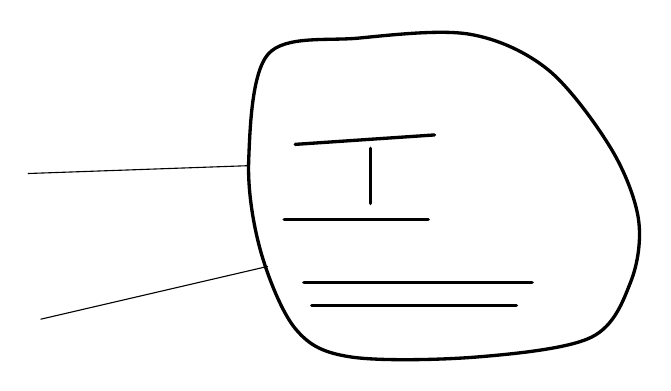
\begin{tikzpicture}[x=1mm,y=1mm,line cap=round,line join=round,font=\scriptsize]
\draw[very thick] plot[smooth cycle, tension=0.55] coordinates {(30.5,-45) (42,-43) (56,-42.5) (66,-47) (74,-57) (77.5,-66) (76.5,-74) (71.5,-81) (57,-83.5) (41,-83.5) (34,-80) (29.5,-70) (28,-58.5)};
\draw[very thick] (33.9,-56.5) -- (51.6,-55.3);
\draw[very thick] (43.5,-57) -- (43.5,-64);
\draw[very thick] (32.5,-66) -- (50.8,-66);
\draw[very thick] (35,-74) -- (64,-74);
\draw[very thick] (36,-77) -- (62,-77);
\draw (0,-60.2) -- (28.1,-59.2);
\draw (1.6,-78.7) -- (30.4,-72);
\end{tikzpicture}
\end{document}
